\documentclass[a4paper]{jpconf}
\usepackage{graphicx}
\usepackage{amsmath,amsfonts,amssymb,amsthm,siunitx,bm}
\numberwithin{equation}{section}

\begin{document}
\title{Electron spin resonance and nuclear magnetic resonance}

\author{2197055V}


\begin{abstract}
Electron spin resonance (ESR) and nuclear magnetic resonance (NMR) are two important spectroscopic techniques for studying properties of materials containing particles or atoms with non-zero magnetic moments. In this experiment, we studied ESR on a sample of Diphenyl-Picryl-Hydrazil (DPPH), a paramagnetic organic molecule with an unpaired $e^-$, by measuring the resonant frequency as a function of externally applied magnetic field in order to determine the sample\textquoteright s $g$-factor, which was found to be $g\textsubscript{DPPH} = 2.02 \pm 0.01$.
Further, we investigated the magnetic properties of ${}^1$H and ${}^{19}$F nuclei in the following substances: glycerine and polystyrene (both of which contain hydrogen), PTFE (which contains fluorine), and polythene, whose composition we wanted to learn about. The experimentally measured $g$-factors were $g\textsubscript{glycerine} = 5.54 \pm 0.03$, $g\textsubscript{polystyrene} = 5.68 \pm 0.01$ and $g\textsubscript{PTFE} = 5.34 \pm 0.01$. Comparison with the results obtained for polythene lead us to postulate the presence of hydrogen in our polythene sample, as confirmed by its chemical formula.

\end{abstract}

\section{Introduction}
Electron spin resonance (ESR), also referred to as electron paramagnetic resonance spectroscopy      % find reference
(EPRS), is an important method for studying paramagnetic chemical substances in which the electrons' magnetic moments don't cancel, such as organic and inorganic free radicals or transition-metal ion complexes. It can provide detailed information relating to the chemical composition and structure of materials, and therefore finds innumerable applications in biology, chemistry, materials science, medicine and pharmacology, to name just a few.

Similarly, nuclear magnetic resonance (NMR) exploits the fact that some nuclei possess a non-zero overall nuclear spin, and hence a magnetic moment, to study the properties of materials containing such nuclei. NMR has widespread use and applications, notably in medical imaging --- it underlies MRI (magnetic resonance imaging).

\section{ESR}
In the first part of the experiment we studied ESR on a sample of Diphenyl-Picryl-Hydrazil (DPPH), which is a paramagnetic organic molecule with a single unpaired $e^-$. The orbital angular momentum of the electron is essentially zero,    % find reference
and hence the molecule\textquoteright s total magnetic moment is solely due to the electron\textquoteright s spin angular momentum. This makes it particularly suitable for ESR experiments.
 
\subsection{Theory}\label{section: theory}
In the absence of any external magnetic fields (i.e.\ for a free $e^-$), the two possible spin states (``spin up'' and ``spin down'') are degenerate, i.e.\ they have the same energy.

However, energy splitting of the two states occurs when the $e^-$ is placed in an external magnetic field. Indeed, the $e^-$'s spin gives rise to a magnetic moment $\bm{\mu}_S$ which interacts with the applied field and possesses a different energy depending on its spatial orientation. A bound $e^-$ in a material, in general, has additionally an orbital angular momentum $\mathbf{L}$ which also contributes to the total magnetic moment. However, in many compounds, including DPPH, the orbital angular momentum is not significant and only the spin needs to be considered for the purposes of ESR. 

According to quantum mechanics, only two orientations of the spin are possible. The magnitude $S$ of the spin vector $\mathbf{S}$ and its two allowed $z$-components $S_z$, where the $z$-axis is defined to lie along the field direction, are respectively given by
\begin{align}
	S &= \lvert\lvert\mathbf{S}\rvert\rvert = \sqrt{s(s+1)}\hbar = \tfrac{\sqrt{3}}{2}\hbar,  \quad \text{and} \nonumber \\
	S_z &= m_s \hbar. \label{eqn: magnetic moment z-projection}
\end{align}
where $s=\tfrac12$ is the spin quantum number, $m_s=\pm\tfrac12$ is the secondary spin quantum number, and $\hbar$ is the reduced Planck\textquoteright s constant.

The associated magnetic moment is
\begin{align}
	\bm{\mu}_S = - g \frac{\mu_B}{\hbar} \mathbf{S} \label{eqn: magnetic moment}
\end{align}
where $g$ is the Land\'e splitting factor, or $g$-factor, which for a free electron has the value $g_e = 2.002319$, and $\mu_B = 9.274 \times 10^{-24} \si{\joule\per\tesla}$ is the Bohr magneton. Note that the magnetic moment points in the opposite direction as the spin~vector~$\mathbf{S}$ due to the electron's negative charge.

A magnetic moment in a magnetic field $\mathbf{B}$ has potential energy
\begin{align}
	E &= - \bm{\mu}_S \cdot \mathbf{B} \nonumber \\
	  &= - (- g \frac{\mu_B}{\hbar} \mathbf{S})\cdot\mathbf{B} \quad \text{substituting in from \eqref{eqn: magnetic moment}}, \nonumber \\
	  &= g \frac{\mu_B}{\hbar}S_z \lvert\lvert \mathbf{B} \rvert\rvert \quad \text{using \eqref{eqn: magnetic moment z-projection}}, \nonumber \\
	  &= g\mu_Bm_sB \label{eqn: potential energy},
\end{align}
where $B$ denotes the magnitude $\lvert\lvert \mathbf{B} \rvert\rvert$ of the magnetic field (so that $\mathbf{B} = B \, \mathbf{e_z}$, where $\mathbf{e_z}$ is the unit vector in the $z$-direction).

Equation \eqref{eqn: potential energy} shows that the two orientations no longer have the same energy --- the one whose magnetic moment is aligned with the field (or equivalently whose spin points in the direction opposite to the field, i.e.\ having $m_s = -\tfrac12$) has a lower potential energy than the one whose magnetic moment is anti-parallel to the field ---, as depicted in figure \ref{fig: energy splitting}. The energy difference between the two levels is 
\begin{equation}
	\Delta E = g \mu_B B. \label{eqn: energy difference}
\end{equation}

In thermal equilibrium, the spins are distributed according to the Boltzmann distribution
\[
    \frac{N_{+\tfrac12}}{N_{-\tfrac12}} = \exp(- \frac{\Delta E}{k_B T}),
\]
where $k_B$ is the Boltzmann\textquoteleft s constant, and $N_{\pm\tfrac12}$ are the number of spins in the higher and lower states respectively. 

If the conditions are such that there are more spins in the lower state than the upper state, transitions can be induced by supplying energy to the sample, e.g.\ by irradiating it with electromagnetic (EM) radiation with the right frequency $\nu$. The energy of an EM wave is given by $E = h \nu$, where $h$ is Planck's constant, so the condition for resonance is
\begin{equation}
	h\nu = g\mu_B B. \label{eqn: resonance condition}
\end{equation}

\begin{figure}[htbp]
	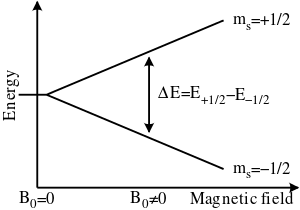
\includegraphics{EPR_splitting.png}
	\caption{Energy splitting of the two spin states of an $e^-$ placed in an external magnetic~field~$\mathbf{B_0}$.}
	\label{fig: energy splitting}
\end{figure}

In a real material, an electron ``feels'' not only the externally applied field, but also the magnetic fields produced by any surrounding magnetic nuclei and/or other electrons, leading to further energy splitting. The effect of the surroundings can be interpreted as a shift in the $g$-value in equation \eqref{eqn: magnetic moment} compared to the free-electron value. The chemical environment of the $e^-$ also has an effect on the shape of the resonance signal and its line width, amongst other things. Thus, ESR can provide a lot of information on the chemical composition and structure of materials. In this experiment, we measured the $g$-value of DPPH.

\subsection{Experimental method}
% Insert figure
The DPPH sample was placed in a uniform magnetic field generated by two parallel vertically-positioned Helmholtz coils (HCs) connected to a DC current supply. The sample was inserted into another coil connected to an RF circuit oscillating at an adjustable frequency $\nu$. This coil provided the energy $h\nu$ needed to flip the $e^-$s spins. The magnetic field produced by the HCs was varied, by changing the current, to identify when the resonance condition \eqref{eqn: resonance condition} was met for a particular (fixed) frequency. The measurement was then repeated for a number of different frequencies. The resonance was detected thanks to a measurable voltage change in the RF circuit, observed using an oscilloscope, that occurred due to the change of the RF coil's permeability when the sample was absorbing energy. (The magnetic field induced in the RF coil was perpendicular to the field of the HCs and was neglected for the purposes of the results analysis).

For an $e^-$ with only two possible spin states, it would be necessary to match the RF frequency and the current in the HCs with considerable accuracy to obtain resonance. Also, once the population of the spin states has been inverted, the sample can no longer absorb more energy before enough electrons have returned to the lower state, so they need to be excited at a rate slower than the relaxation time (the time needed for the electrons to de-excite and return to thermal equilibrium via spin-spin and spin-lattice interactions). The solution to both problems was to superimpose a ($50 \si{\hertz}$) modulation (AC) current on the DC component going into the HCs, resulting in a sinusoidally-varying modulation magnetic field. The total field $\mathbf{B}_{total}$ was then the superposition of the two, and thus oscillated around a central value $B_0$. If the resonance condition \eqref{eqn: resonance condition} was satisfied for some value of $\mathbf{B}_{total}$ during this oscillation, a resonance signal was observed, twice during the cycle at symmetric positions (provided that the phase lag between the modulation signal and the sample response signal was correctly accounted for). By adjusting the DC current, it was possibly to make the resonance occur precisely at the point when the modulation field dropped to zero and the field was equal simply to $B_0$, i.e.\ it was the $B_0$ that satisfying \eqref{eqn: resonance condition} for the given frequency.

The value of $B_0$ could be deduced from the DC current $I_0$ in the coils --- we created a calibration curve of $B_0$ as a function of $I_0$ using a Hall probe sensor to measure the magnetic field in the centre of the coil set-up.

\subsection{Results}
The following two sections present the results that we obtained.

\subsubsection{Helmholtz coils calibration.}
The direct current going through the Hemlhotz coils was varied and the magnetic field $B_0$ at the centre of the coils was recorded. We observed quite large fluctuations of the field for a given current, and therefore 5 different readings were taken and averaged. For the purposes of error analysis, the uncertainty in the mean was then taken to be half the spread of the observed values (as there weren't enough readings to justify using the formula for the standard error in the mean). For the current, the measurement uncertainty was taken to be half the smallest scale division. 

We subsequently performed a weighted straight-line fit to the data. Figure \ref{fig: HC calibration curve} shows the resulting calibration curve with uncertainties indicated by error bars. This curve was used in the second part to convert between measured current and magnetic field applied to the sample. We used the MATLAB's built-in function \texttt{polyval} to estimate the uncertainties in the values of $B_0$ predicted by the curve for a given $I$, based on the goodness of fit.

We obtained 
\[
	B_0 = (3.73 \pm 0.01) I + (0.03 \pm 0.01),
\]
where $I$ is in $\si{\ampere}$ and $B_0$ is in $\si{\milli\tesla}$.

\begin{figure}[htbp]
	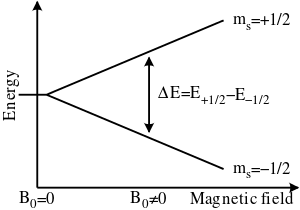
\includegraphics{EPR_splitting.png}
	\label{fig: HC calibration curve}
\end{figure}



\subsubsection{Measurement of the $g$-factor of DPPH.}
The frequency in the RF oscillator circuit was varied in steps of $5 \si{\mega\hertz}$, and for each frequency, the current in the Helmholtz coils was scanned over the range $0.1 \si{\ampere}$ to $1.2 \si{\ampere}$ to find the resonance. For a given frequency, the measurement was repeated multiple times to get an idea of the uncertainty in the resonant current. Figure \ref{fig: DPPH resonance} shows the resonance frequency as a function of the field.

\begin{figure}[htbp]
	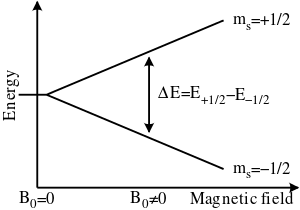
\includegraphics{EPR_splitting.png}
	\label{fig: DPPH resonance}
\end{figure}

\subsection{Analysis}
According to equation \eqref{eqn: resonance condition}, the plot of frequency $\nu$ against magnetic field $B_0$ should be a straight line with gradient 
\[
	\frac{\nu}{B_0} = \frac{g_{\textsubscript{DPPH}} \mu_B}{h},
\]
which implies
\begin{equation} \label{eqn: gradient}
	g_{\textsubscript{DPPH}} = \left(\frac{h}{\mu_B}\right) \left(\frac{\nu}{B_0}\right). 
\end{equation}
	
From the weighted straight-line fit to our data shown in figure \ref{fig: DPPH resonance}, we have
\[
	\left(\frac{\nu}{B_0}\right) = 28.24 \pm 0.07 \; \si{\mega\hertz\per\milli\tesla}.
\]

Substituting into \eqref{eqn: gradient} yields 
\[
	g_{\textsubscript{DPPH}} = 2.02 \pm 0.01,
\] 
(where the uncertainty in the final value has been computed, given that $h$ and $\mu_B$ are exact values, simply by multiplying the error in the gradient by $h / \mu_B$ ).

\subsection{Discussion}
For a pair of Helmholtz coils separated by a distance equal to their radius, electromagnetic theory predicts that the value of the field at the centre should obey approximately
\[
	B_0 = \mu_0 \left(\frac45\right)^{\tfrac32} \frac{n}{r} I,
\]
where $\mu = 4\pi\times10^{-7} \; \si{\volt\s\ampere\tothe{-1}\meter\tothe{-1}}$, $n$ is the number of turns per coil, and $r$ is their radius.

This shows that the expected relationship between $I$ and $B_0$ was linear, as confirmed by our data (see figure \ref{fig: HC calibration curve}).
However, for our particular coils, the expected value of the gradient was $4.23$, which does not agree with the value that we obtained experimentally, i.e.\ $3.73 \pm 0.01$. This could be due to the fact that the separation of the coils might not have been exactly equal to their radius. Due to such possible differences in our set-up from the idealised case, we used the experimentally obtained calibration curve in the subsequent sections, not the theoretical one. Any error in the calibration curve therefore represents a systematic error in the results obtained for DPPH. 

Possible sources of error were the difficulty in making sure that the Hall probe was oriented exactly perpendicular to the measured field (i.e.\ parallel to the coils), and that it was located at the exact position where the sample was later inserted. We also couldn't be sure whether the Hall probe itself was calibrated correctly (as we didn't obtain the expected result when we checked with a standard magnet), and whether we zeroed it at a point with no magnetic field. This could have introduced a systematic offset. A source statistical errors were the random fluctuations in the magnetic field and in the response of the probe over time (e.g.\ due to warming up of the equipment).

Our measurement of the DPPH resonance confirmed the linear relationship predicted by \eqref{eqn: resonance condition} for the magnetic field and the resonance frequency. This shows that, indeed, an energy splitting occurs when the sample is placed in an external field, that this creates two separate energy levels such that the energy difference between them scales linearly with the applied field, and that energy transitions can be induced by supplying EM energy of the correct frequency. 

The accepted value for the $g$-factor of DPPH is
\[
	g_{\textsubscript{DPPH, th}} = 2.0036.
\]
Our value lies within $2\sigma$ of this value, and is therefore in reasonable agreement.
Compare this with the theoretical value for the $g$-factor due to the spin of a free $e^-$
\[
	g_e = 2.002319.
\]
This is slightly different from both the accepted and our experimental value for $g_{\textsubscript{DPPH}}$, which as explained in the (\ref{section: theory}) theory section can be due to the effect of the chemical surrounding of the unpaired $e^-$ in DPPH. Nevertheless, the values are relatively close, showing in particular that the assumption that we can neglect the orbital angular momentum of the $e^-$ and attribute the molecule's magnetic moment solely to the spin angular momentum was largely justified.

An increase in the precision of our measurements could have been achieved by taking further repeated measurements for a given set of conditions in order to deal with statistical errors due to random fluctuations, but also by using stronger $\mathbf{B}$ field, thus increasing the energy difference between the two spin states and hence reducing the relative uncertainty in this difference, and/or by operating at lower temperatures, both of which could possibly result in a sharper resonance signal (i.e.\ a reduced line width).


\section{NMR} 
\subsection{Theory}
\subsection{Experimental method}
\subsection{Results}
\subsubsection{Electromagnet calibration}
\subsubsection{Measurement of the $g$-factors}
\subsection{Analysis}

\subsection{Discussion}

\section{Conclusion}

\section*{References}
\begin{thebibliography}{9}
\bibitem{iopartnum} 
\end{thebibliography}

\end{document}


